\documentclass[a4paper,12pt]{article}
\usepackage{amssymb}
\usepackage{amsfonts}

% Кодировка и язык
\usepackage[utf8]{inputenc}
\usepackage[russian]{babel}

% Математические пакеты
\usepackage{amsmath,amsfonts,amssymb}
%Таблицы
\usepackage{array}
\usepackage{booktabs} % Для более красивых горизонтальных линий в таблицах
\usepackage{graphicx}
\usepackage{array}
\usepackage{booktabs}
% Геометрия страницы
\usepackage{geometry}
\geometry{top=2cm, bottom=2cm, left=2.5cm, right=2.5cm}

% Гиперссылки (лучше загружать последним)
\usepackage{hyperref}


% Настройки заголовка
\title{Домашнее задание}
\author{Студент: \textbf{Ростислав Лохов}}
\date{\today}

\begin{document}

% Титульный лист
\begin{titlepage}
    \centering
    \vspace*{1cm}

    \Huge
    \textbf{Домашнее задание}

    \vspace{0.5cm}
    \LARGE
    По курсу: \textbf{Экономика}

    \vspace{1.5cm}

    \textbf{Студент: Ростислав Лохов}

    \vfill

    \Large
    АНО ВО Центральный университет\\
    \vspace{0.3cm}
    \today

\end{titlepage}

% Содержание
\tableofcontents
\newpage

% Основной текст
\section{Сине-Красный уровень}


\subsection{Задача 1}
\begin{enumerate}
    \item Пандемия(закрытые границы, ограничения на передвижения)-> Сокращение притока трудовых мигрантов в Москву/запрет на выход на улицу -> Уменьшение предложения рабочей силы -> Возникновение дефицита дворников -> Управляющая компания чистит снег само
    \item Совокупность экономических факторов(рост арендных ставок, изменение спроса, конкуренция) привели к тому, что магазины не смогли адаптироваться. Рост турпотока скорее всего повлиял к тому, что повысился спрос на коммерческую недвижимость.
    \item Орангутанги - дело тонкое, их исчезновение - результат экономического стимула к производству пальмового масла, которое ведет к уничтожению лесов. Хороший способ - экономические стимулы за другую деятельность, чтобы сделать экономически выгодным сохранение орангутангов.
    \item Во всех трех случаях рыночные ситуации и экономические стимулы определяют результаты.
\end{enumerate}

\subsection{Задача 2}
\begin{enumerate}
    \item КПВ Робинзона: Альтернативные издержки Робинзона: 2.5 банана за рыбу и 0.4 рыбы за банан.
    \item КПВ Пятницы: Альтернативные издержки Пятницы: 3.33 банана за рыбу и 0.3 рыбы за банан.
    \item Абсолютным приемуществом обладает Пятница т.к больше производственные мощности по обоим продуктам
    \item Сравнительным приемуществом обладает пятница в бананах, а Робинзон - в рыбах.
    \item Продавать бананы будет Пятница Робинзону.
\end{enumerate}

\subsection{Задача 3}
\begin{enumerate}
    \item Да. т.к конфликт обусловлен дефицитом гаражей, которое необходимо распределить. Т.е выбор в условиях ограниченности ресурсов - область экономического анализа..
    \item Что производить, как производить и кому производить(скорее кто не получит)?
    \item Профессор и его научные сотрудники разгружали овощи на овощной базе. Они оказались там потому, что в условиях плановой экономики предприятия привлекались к выполнению работ не связанных с основной деятельностью
    \item Альтернативные издержки - время и усилия, которые они могли бы потратить на свою основную работу – научные исследования.
    \item Такое возможно поскольку главным показателем в плановой экономике является выполнение плана спущенного сверху. Также отсутствие рыночных механизмов и стимулов для эффективного использования ресурсов.
\end{enumerate}

\subsection{Задача 4}
\begin{enumerate}
    \item Ограниченность ресурсов - прокладывание и обслуживание резервных труб экономически нецелесообразно
    \item Альтернативные издержки - вторая труба здесь, а где-то без трубы
    \item Экономическая нецелесообразность.
    \item Неэффективное использование ресурсов.
\end{enumerate}

\begin{enumerate}
    \item Проблема не в количестве, а в надобности.
    \item Базовое увеличение производства важно, но не всего подряд
    \item Ресурсы ограничены, всего не произвести много.
    \item Увеличение производства всего не приведет к получению всего.
\end{enumerate}

\subsection{Задача 5}
\begin{enumerate}
    \item Абсолютное преимущество у отца в зарабатывании деднег, у бабушки - в времени и гибкости графика
    \item Сравнительное преимущество - бабушка(упущенное время на вязание, против упущенных заработанных денег у папы)
\end{enumerate}

\subsection{Задача 6}
А
\begin{enumerate}
    \item Азилия может вырастить 50 тонн кукурузы либо 20 тонн риса (2.5 тонны кукурузы за тонну риса и 0.4 тонны риса за тонну кукурузы)
    \item Бомерика может вырастить 30 тонн кукурузы либо 80 тонн риса (0.375 тонны кукурузы за тонну риса и 2.666 тонны риса за тонну кукурузы)
\end{enumerate}
Б
\begin{enumerate}
    \item Абсолютное преимущество в производстве кукурузы - у Азилии. В производстве риса - у Бомерики.
    \item Сравнительное преимущество в производстве кукурузы - у Бомерики. В производстве риса - у Азилии.
\end{enumerate}
В
Cоставим функцию и проверим
\[
Corn(Rice) = 
\begin{cases}
    80 - 0.375Rice & 0 \le Rice \le 80 \\
    250 - 2.5Rice, & 80 \le y \le 100
\end{cases}
\]

\begin{enumerate}
    \item Да, под
    \item Нет, над
    \item Нет, над
    \item Нет, над
    \item Да, на
    \item Нет, над
\end{enumerate}

\section{Черный уровень}
\subsection{Задача 1}

\begin{enumerate}
    \item Средняя стоимость аренды - 275 тысяч. Т.е живя в своей квартире человек отказывается от возможности получать пассивный доход в размере около 275 тыс рублей
    \item Средняя стоимость квартиры - 60 млн рублей. Ставка по вкладам - 23 среднее. Доход от вкладов - 1.1 млн в месяц. Таким образом издержки - 1.1 млн рублей без учета стоимости аренды.
    \item Средняя стоимость такой же квартиры, но уже на окружности мкада - около 25 млн рублей. Разница - 35 млн. Доход в месяц - 700к рублей. 
    \item Минусы - ключевая ставка крайне высокая и нестабильная.
\end{enumerate}

\subsection{Задача 2}
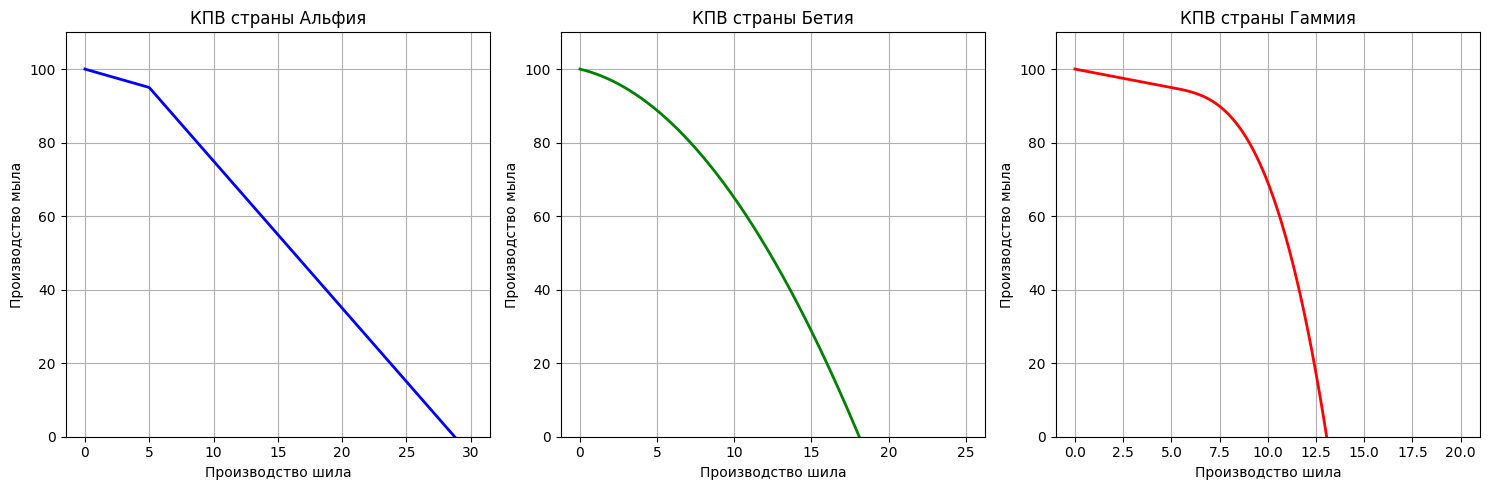
\includegraphics[scale=0.45]{graphs/1.1.png}

коэффициенты взяты ради примера.

\subsection{Задача 3}
\begin{enumerate}
    \item Азилия - 2 барреля за смартфон ,0.5 смартфона за баррель. Брамерика - 4 баррели за смартфон, 0.25 смартфона за баррель.
    \item Сравнительное преимущество имеет Азилия в смартфонах, Брамерика - в нефти.
    \item 2 барреля нефти < цены смартфона в Азилии. 4 барреля нефти дороже чем 1 смартфон. Азилия торгует смартфонами, Брамерика - нефтью.
    \item А)На мировом ранке 1 смартфон = 2.5 барреля нефти. В таком случае Брамерике выгодно продавать нефть, Азилии - смартфоны.
    \item Б) 1 смартфон = 3.2 барреля нефти. Азилии выгодно экспортировать смартфоны, Брамерике тоже выгодно, однако меньше, чем в пункте А.
    \item 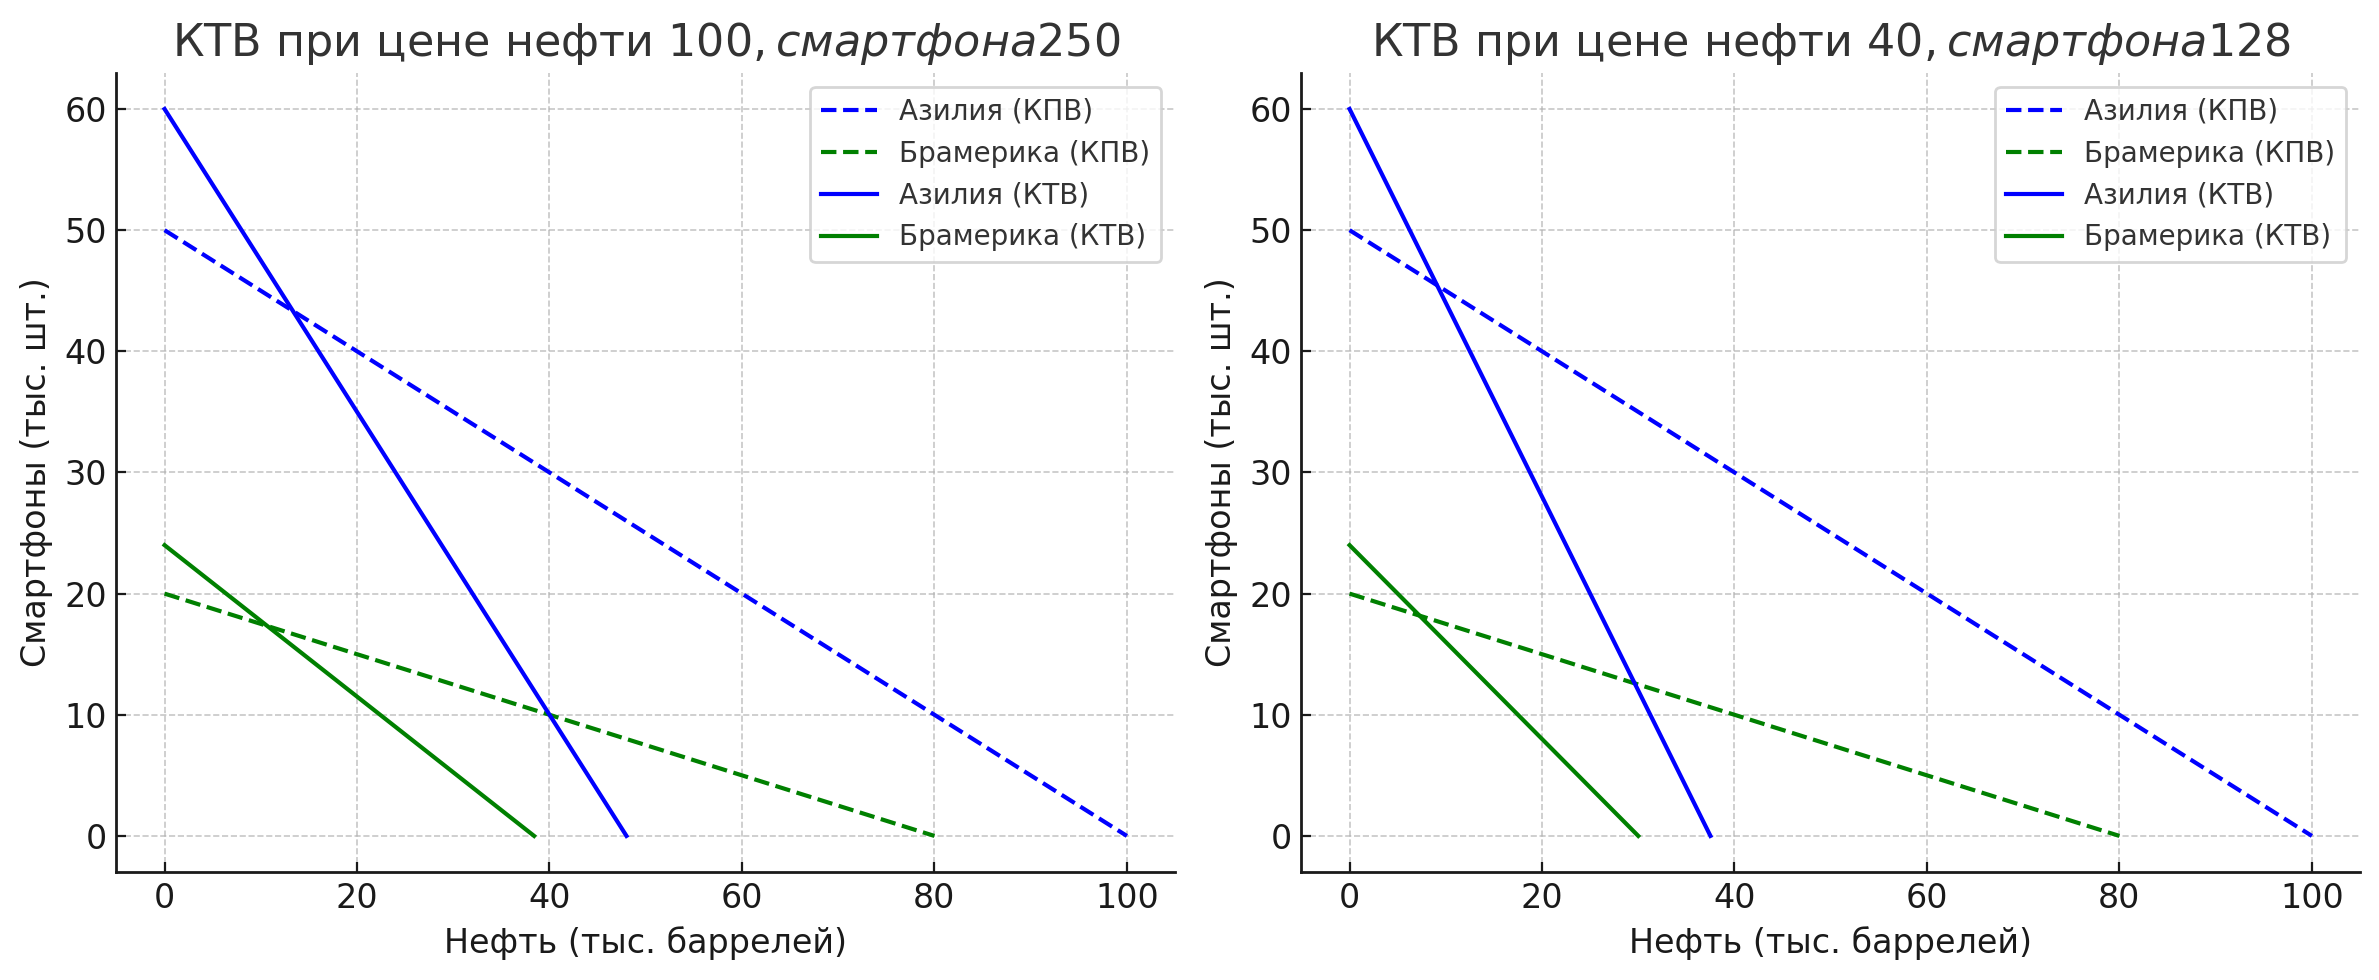
\includegraphics[scale=0.5]{graphs/1.2.png}
\end{enumerate}

\end{document}